
\section{Testing}

\vspace{20mm}


\Huge{\textbf{Testing}}

\vspace{20mm}


\begin{abstract}

    This chapter is dedicated to representing the Testing of the system
    through a variety of different testing techniques. These testing techniques will show
    various aspects of the system responses, including the relationships between the
    various entities, the relationships between the entities and the database responses,
    and the relationships between the entities and the user interface.
    The positive flow and development of states would also be demonstrated in the test cases.


\end{abstract}

\vspace{20mm}

\large{\textbf{Outline}}

\begin{center}
    \begin{itemize}
        \item Test Case Specification
        \item Black Box Testing
        \item Use Case Testing
        \item White Box Testing
        \item Performance Testing
        \item Load Testing
        \item Stress Testing
        \item Regression Testing
    \end{itemize}
\end{center}
\pagebreak


% Test Case Specification
\subsection{Test Case Specification}
%Test Case Specification
%File path

% Black Box Testing
\subsection{ Black Box Testing}
Black Box testing is the Software testing method which is used to test the software without knowing the internal workings of the software.
Black box testing helps to find the gaps in functionality, usability and other features of the software. This form of testing is used to find the bugs in the software.
It improves software quality and reducesthe time to market. This form of testing mitigates the risk of software defects at the user's end.

Black-box testing attempts to find errors in the following categories:
\begin{itemize}
    \item Incorrect or missing functions.
    \item Interface errors.
    \item Errors in data structures or external database access.
    \item Behavior or performance errors.
    \item Initialization and termination errors.
\end{itemize}

Typical Black-box test design Techniques include:
\begin{itemize}
    \item Equivalence Partiotioning
    \item Boundary Value Analysis
    \item Decision Table
    \item State Transition Tables
    \item Use Case analysis
\end{itemize}


%Equivalence Partition
\subsubsection*{Equivalence Partitioning}

\subsubsubsection*{Register}
\textbf{ Register}
\begin{table}[]
    \centering
    \begin{tabular}{lllll}
        Variable & Valid Classes                                                                                                                                                                                                & Invalid Classes                                                                                                  &  & \\
        Name     & \begin{tabular}[c]{@{}l@{}}1. Compulsory field\\ 2. Contain alphabets\\ [a-z A-Z], numeric values [0-9], and special\\ character [@].\end{tabular}                                                           & 1. Empty Field                                                                                                   &  & \\
        Email    & \begin{tabular}[c]{@{}l@{}}1. Compulsory field\\ 2. Contain alphabets\\ [a-z A-Z], numeric\\ values [0-9] and special\\ character [@].\\ 3. Valid email address.\end{tabular}                                & \begin{tabular}[c]{@{}l@{}}1. Empty Field\\ 2. Special characters\\ except [@] is not\\ acceptable.\end{tabular} &  & \\
        Password & \begin{tabular}[c]{@{}l@{}}1. Compulsory field\\ 2. Length should be 8 or\\ greater than 8characters.\\ 3. May contain symbols,\\ alphabets [a-z A-Z],\\ digits [0-9] and special\\ characters.\end{tabular} & \begin{tabular}[c]{@{}l@{}}1. Empty Field\\ 2. Length smaller than 8\\ characters.\end{tabular}                  &  &
    \end{tabular}
\end{table}

\subsubsubsection*{Login}
\textbf{ Login}
\begin{table}[]
    \centering
    \begin{tabular}{lllll}
        Variable & Valid Classes                                                                                                                                                                                                & Invalid Classes                                                                                                  &  & \\
        Email    & \begin{tabular}[c]{@{}l@{}}1. Compulsory field\\ 2. Contain alphabets\\ [a-z A-Z], numeric\\ values [0-9] and special\\ character [@].\\ 3. Valid email address.\end{tabular}                                & \begin{tabular}[c]{@{}l@{}}1. Empty Field\\ 2. Special characters\\ except [@] is not\\ acceptable.\end{tabular} &  & \\
        Password & \begin{tabular}[c]{@{}l@{}}1. Compulsory field\\ 2. Length should be 8 or\\ greater than 8characters.\\ 3. May contain symbols,\\ alphabets [a-z A-Z],\\ digits [0-9] and special\\ characters.\end{tabular} & \begin{tabular}[c]{@{}l@{}}1. Empty Field\\ 2. Length smaller than 8\\ characters.\end{tabular}                  &  &
    \end{tabular}
\end{table}

\subsubsubsection*{Update Profile}
\textbf{ Update Profile}
\begin{table}[]
    \centering
    \begin{tabular}{lllll}
        Variable         & Valid Classes                                                                                                                                                                                                & Invalid Classes                                                                                                  &  & \\
        Name             & \begin{tabular}[c]{@{}l@{}}1. Compulsory field\\ 2. Contain alphabets\\ [a-z A-Z], numeric values [0-9], and special\\ character [@].\end{tabular}                                                           & 1. Empty Field                                                                                                   &  & \\
        Email            & \begin{tabular}[c]{@{}l@{}}1. Compulsory field\\ 2. Contain alphabets\\ [a-z A-Z], numeric\\ values [0-9] and special\\ character [@].\\ 3. Valid email address.\end{tabular}                                & \begin{tabular}[c]{@{}l@{}}1. Empty Field\\ 2. Special characters\\ except [@] is not\\ acceptable.\end{tabular} &  & \\
        Password         & \begin{tabular}[c]{@{}l@{}}1. Compulsory field\\ 2. Length should be 8 or\\ greater than 8characters.\\ 3. May contain symbols,\\ alphabets [a-z A-Z],\\ digits [0-9] and special\\ characters.\end{tabular} & \begin{tabular}[c]{@{}l@{}}1. Empty Field\\ 2. Length smaller than 8\\ characters.\end{tabular}                  &  &
        Confirm Password & \begin{tabular}[c]{@{}l@{}}1. Compulsory field\\ 2. Length should be 8 or\\ greater than 8characters.\\ 3. May contain symbols,\\ alphabets [a-z A-Z],\\ digits [0-9] and special\\ characters.\end{tabular} & \begin{tabular}[c]{@{}l@{}}1. Empty Field\\ 2. Length smaller than 8\\ characters.\end{tabular}                  &  &
    \end{tabular}
\end{table}

\subsubsubsection*{Add Project}
\textbf{ Update Profile}
\begin{table}[]
    \centering
    \begin{tabular}{lllll}
        \hline
        Variable     & Valid Classes                                                                                                                                                                   & Invalid Classes                                                                                                  &  & \\ \hline
        Project Name & \begin{tabular}[c]{@{}l@{}}1. Compulsory field\\ 2. Contain alphabets [a-z\\ A-Z], numeric values\\ [0-9].\end{tabular}                                                         & \begin{tabular}[c]{@{}l@{}}1. Empty Field\\ 2. Submitting Error\end{tabular}                                     &  & \\
        Organization & \begin{tabular}[c]{@{}l@{}}1. Compulsory field\\ 2. Contain alphabets\\ [a-z A-Z], numeric\\ values [0-9] and special\\ character [@].\\ 3. Valid email address.\end{tabular}   & \begin{tabular}[c]{@{}l@{}}1. Empty Field\\ 2. Special characters\\ except [@] is not\\ acceptable.\end{tabular} &  & \\
        Actors       & \begin{tabular}[c]{@{}l@{}}1. Compulsory field\\ 2. May contain symbols,\\ alphabets [a-z A-Z],\\ digits [0-9] and special\\ characters.\\ 3. Select Type of Actor\end{tabular} & \begin{tabular}[c]{@{}l@{}}1. Empty Field\\ 2. Length smaller than 8\\ characters.\end{tabular}                  &  &
        Usecases     & \begin{tabular}[c]{@{}l@{}}1. Compulsory field\\ 2. May contain symbols,\\ alphabets [a-z A-Z],\\ digits [0-9] and special\\ characters.\\ 3. Select Type of Actor\end{tabular} & \begin{tabular}[c]{@{}l@{}}1. Empty Field\\ 2. Length smaller than 8\\ characters.\end{tabular}                  &  &
    \end{tabular}
\end{table}

\subsubsubsection*{Add Organization}
\textbf{ Update Profile}
\begin{table}[]
    \centering
    \begin{tabular}{lllll}
        \hline
        Variable       & Valid Classes                                                                                                           & Invalid Classes                                                              &  & \\ \hline
        Company Name   & \begin{tabular}[c]{@{}l@{}}1. Compulsory field\\ 2. Contain alphabets [a-z\\ A-Z], numeric values\\ [0-9].\end{tabular} & \begin{tabular}[c]{@{}l@{}}1. Empty Field\\ 2. Submitting Error\end{tabular} &  & \\
        Company Slogan & \begin{tabular}[c]{@{}l@{}}1. Compulsory field\\ 2. Contain alphabets [a-z\\ A-Z], numeric values\\ [0-9].\end{tabular} & \begin{tabular}[c]{@{}l@{}}1. Empty Field\\ 2. Submitting Error\end{tabular} &  & \\
    \end{tabular}
\end{table}

\subsubsection*{UCP Estimation}
\textbf{UCP Estimation}
\begin{table}[]
    \centering
    \begin{tabular}{lllll}
        \hline
        Variable     & Valid Classes                                                                                              & Invalid Classes                                                              &  & \\ \hline
        UCP variable & \begin{tabular}[c]{@{}l@{}}1. Compulsory field\\ 2. Contain alphabets numeric values\\ [0-9].\end{tabular} & \begin{tabular}[c]{@{}l@{}}1. Empty Field\\ 2. Submitting Error\end{tabular} &  &
    \end{tabular}
\end{table}

\subsubsection*{Delphi Estimation}
\textbf{UCP Estimation}
\begin{table}[]
    \centering
    \begin{tabular}{lllll}
        \hline
        Variable                   & Valid Classes                                                                                              & Invalid Classes                                                              &  & \\ \hline
        Delphi variable            & \begin{tabular}[c]{@{}l@{}}1. Compulsory field\\ 2. Contain alphabets numeric values\\ [0-9].\end{tabular} & \begin{tabular}[c]{@{}l@{}}1. Empty Field\\ 2. Submitting Error\end{tabular} &  &
        Delphi array of estimation & \begin{tabular}[c]{@{}l@{}}1. Compulsory field\\ 2. Contain alphabets numeric values\\ [0-9].\end{tabular} & \begin{tabular}[c]{@{}l@{}}1. Empty Field\\ 2. Submitting Error\end{tabular} &  &
        Delphi result              & \begin{tabular}[c]{@{}l@{}}1. Compulsory field\\ 2. Contain alphabets numeric values\\ [0-9].\end{tabular} & \begin{tabular}[c]{@{}l@{}}1. Empty Field\\ 2. Submitting Error\end{tabular} &  &
    \end{tabular}
\end{table}

\subsubsection*{Machine Learning Estimation}
\textbf{UCP Estimation}
\begin{table}[]
    \centering
    \begin{tabular}{lllll}
        \hline
        Variable                & Valid Classes                                                                                              & Invalid Classes                                                              &  & \\ \hline
        Machine variable        & \begin{tabular}[c]{@{}l@{}}1. Compulsory field\\ 2. Contain alphabets numeric values\\ [0-9].\end{tabular} & \begin{tabular}[c]{@{}l@{}}1. Empty Field\\ 2. Submitting Error\end{tabular} &  &
        Machine Result Variable & \begin{tabular}[c]{@{}l@{}}1. Compulsory field\\ 2. Contain alphabets numeric values\\ [0-9].\end{tabular} & \begin{tabular}[c]{@{}l@{}}1. Empty Field\\ 2. Submitting Error\end{tabular} &  &
    \end{tabular}
\end{table}


\subsubsection*{Esembled Module Estimation}
\textbf{UCP Estimation}
\begin{table}[]
    \centering
    \begin{tabular}{lllll}
        \hline
        Variable                & Valid Classes                                                                                              & Invalid Classes                                                              &  & \\ \hline
        Esemble variable        & \begin{tabular}[c]{@{}l@{}}1. Compulsory field\\ 2. Contain alphabets numeric values\\ [0-9].\end{tabular} & \begin{tabular}[c]{@{}l@{}}1. Empty Field\\ 2. Submitting Error\end{tabular} &  &
        Esemble Result Variable & \begin{tabular}[c]{@{}l@{}}1. Compulsory field\\ 2. Contain alphabets numeric values\\ [0-9].\end{tabular} & \begin{tabular}[c]{@{}l@{}}1. Empty Field\\ 2. Submitting Error\end{tabular} &  &
    \end{tabular}
\end{table}




% Use Case Testing
\subsection{Use Case Testing}

% White Box Testing
\subsection{ White Box Testing}
In white-box testing an internal perspective of the system, as well as programming skills, are used to
design test cases. The tester chooses inputs to exercise paths through the code and determine the
expected outputs.

% Cyclomatic Testing

\subsubsection{ Cyclomatic Testing}
Cyclomatic complexity is a software metric used to indicate the complexity of a program. It is a
quantitative measure of the number of linearly independent paths through a program`s source code.

\begin{figure}[H]

    \centering
    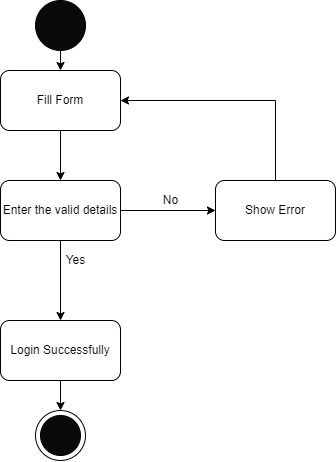
\includegraphics[scale=0.7]{./diagrams/Activity Diagram/ad-01.png}
    \caption{Activity diagram of UC-1}
    \label{fig:act-01}

\end{figure}

\textbf{Cyclomatic Complexity}

M= E-N + 2(P)

E= number of edges

N= number of nodes

P= number of paths

E= 6,
N= 6,
P= 1,

M= 6-6+2(1)= 2

\begin{figure}[H]
    \centering
    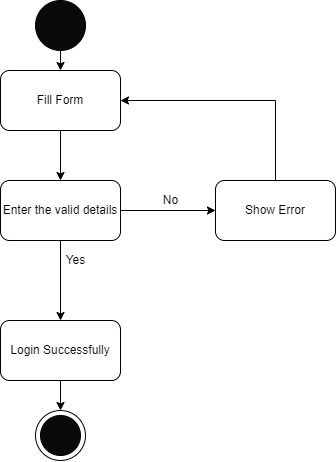
\includegraphics[scale=0.7]{./diagrams/Activity Diagram/ad-02.png}
    \caption{Activity diagram of UC-2}
    \label{fig:act-02}

\end{figure}

\textbf{Cyclomatic Complexity}

M= E-N + 2(P)

E= number of edges

N= number of nodes

P= number of paths

E= 6,
N= 6,
P= 1,

M= 6-6+2(1)= 2

\begin{figure}[H]
    \centering
    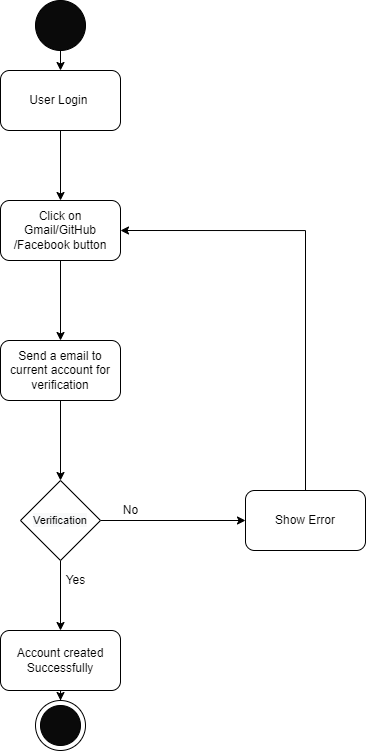
\includegraphics[scale=0.7]{./diagrams/Activity Diagram/ad-03.png}
    \caption{Activity diagram of UC-3}
    \label{fig:act-03}

\end{figure}

\textbf{Cyclomatic Complexity}

M= E+N + 2(P)

E= number of edges

N= number of nodes

P= number of paths

E= 8,
N= 8,
P= 1,

M= 8-8+2(1)= 2

\begin{figure}[H]
    \centering
    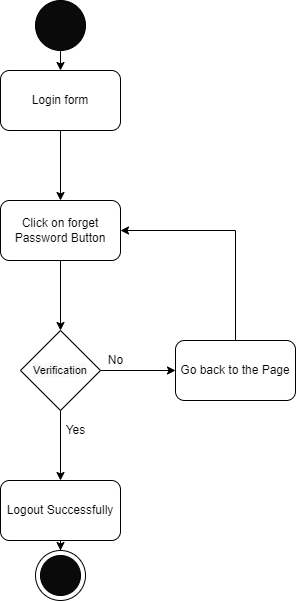
\includegraphics[scale=0.7]{./diagrams/Activity Diagram/ad-04.png}
    \caption{Activity diagram of UC-4}
    \label{fig:act-04}

\end{figure}

\textbf{Cyclomatic Complexity}

M= E+N + 2(P)

E= number of edges

N= number of nodes

P= number of paths

E= 7,
N= 7,
P= 1,

M= 7-7+2(1)= 2

\begin{figure}[H]
    \centering
    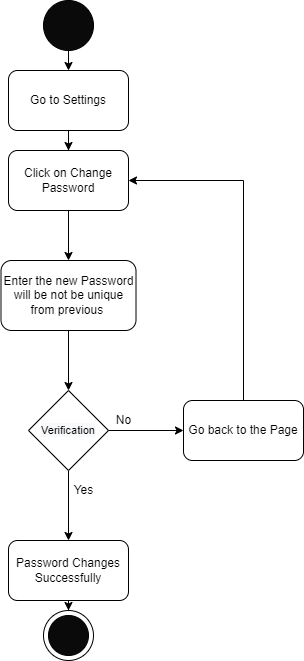
\includegraphics[scale=0.7]{./diagrams/Activity Diagram/ad-05.png}
    \caption{Activity diagram of UC-7}
    \label{fig:act-05}

\end{figure}


\textbf{Cyclomatic Complexity}

M= E+N + 2(P)

E= number of edges

N= number of nodes

P= number of paths

E= 8,
N= 8,
P= 1,

M= 8-8+2(1)= 2

\begin{figure}[H]
    \centering
    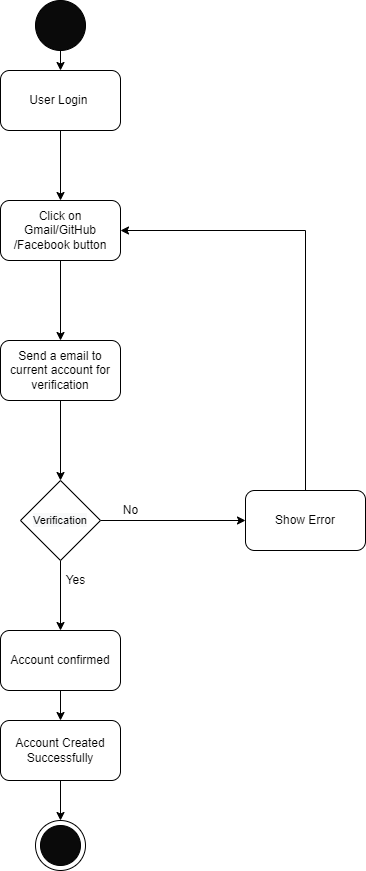
\includegraphics[scale=0.6]{./diagrams/Activity Diagram/ad-06.png}
    \caption{Activity diagram of UC-6}
    \label{fig:act-06}

\end{figure}


\textbf{Cyclomatic Complexity}
\textbf{Cyclomatic Complexity}

M= E+N + 2(P)

E= number of edges

N= number of nodes

P= number of paths

E= 9,
N= 9,
P= 1,

M= 9-9+2(1)= 2

\begin{figure}[H]
    \centering
    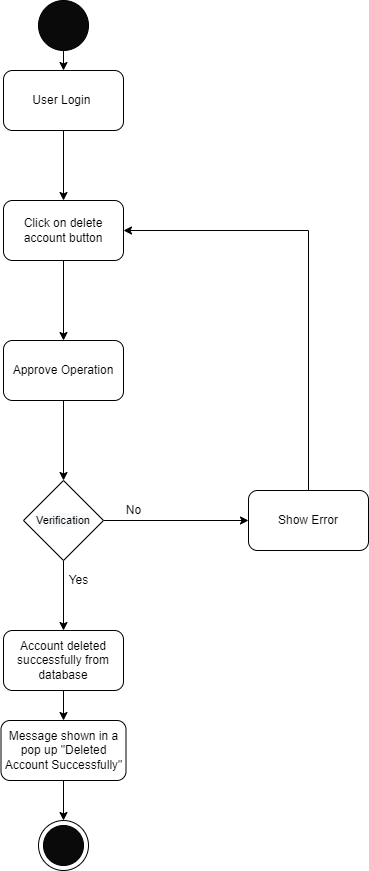
\includegraphics[scale=0.6]{./diagrams/Activity Diagram/ad-07.png}
    \caption{Activity diagram of UC-7}
    \label{fig:act-07}

\end{figure}


\textbf{Cyclomatic Complexity}

M= E+N + 2(P)

E= number of edges

N= number of nodes

P= number of paths

E= 9,
N= 9,
P= 1,

M= 9-9+2(1)= 2

\begin{figure}[H]
    \centering
    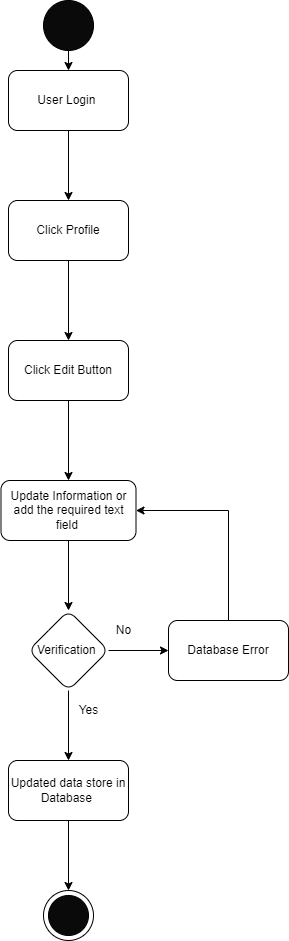
\includegraphics[scale=0.6]{./diagrams/Activity Diagram/ad-08.png}
    \caption{Activity diagram of UC-8}
    \label{fig:act-08}

\end{figure}


\textbf{Cyclomatic Complexity}


M= E+N + 2(P)

E= number of edges

N= number of nodes

P= number of paths

E= 9,
N= 9,
P= 1,

M= 9-9+2(1)= 2

\begin{figure}[H]
    \centering
    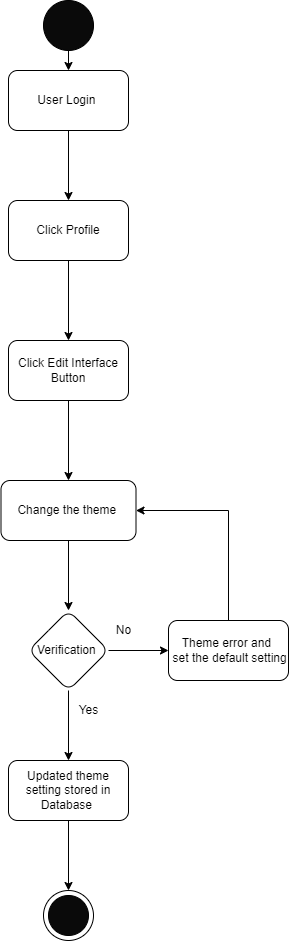
\includegraphics[scale=0.6]{./diagrams/Activity Diagram/ad-09.png}
    \caption{Activity diagram of UC-9}
    \label{fig:act-09}

\end{figure}


\textbf{Cyclomatic Complexity}

M= E+N + 2(P)

E= number of edges

N= number of nodes

P= number of paths

E= 9,
N= 9,
P= 1,

M= 9-9+2(1)= 2

\begin{figure}[H]
    \centering
    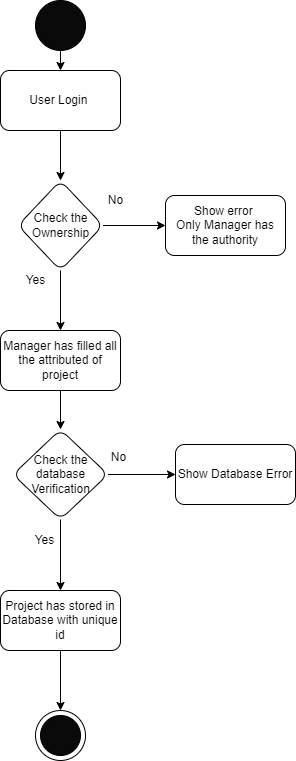
\includegraphics[scale=0.7]{./diagrams/Activity Diagram/ad-10.png}
    \caption{Activity diagram of UC-10}
    \label{fig:act-10}

\end{figure}


\textbf{Cyclomatic Complexity}
M= E+N + 2(P)

E= number of edges

N= number of nodes

P= number of paths

E= 8,
N= 9,
P= 1,

M= 8-9+2(1)= 1

\begin{figure}[H]
    \centering
    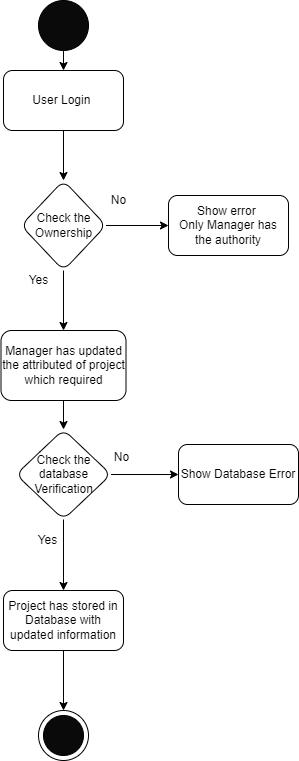
\includegraphics[scale=0.7]{./diagrams/Activity Diagram/ad-11.png}
    \caption{Activity diagram of UC-11}
    \label{fig:act-11}

\end{figure}


\textbf{Cyclomatic Complexity}

M= E+N + 2(P)

E= number of edges

N= number of nodes

P= number of paths

E= 8,
N= 9,
P= 1,

M= 8-9+2(1)= 1

\begin{figure}[H]
    \centering
    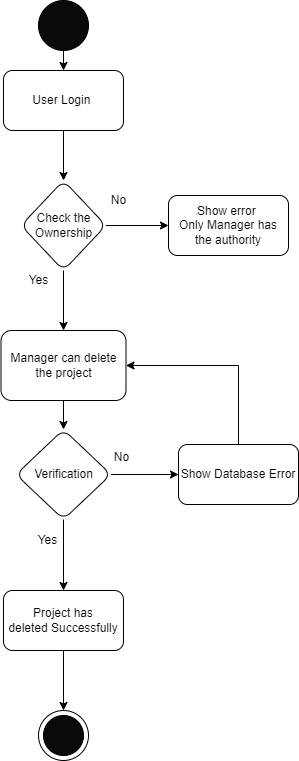
\includegraphics[scale=0.7]{./diagrams/Activity Diagram/ad-12.png}
    \caption{Activity diagram of UC-12}
    \label{fig:act-12}

\end{figure}


\textbf{Cyclomatic Complexity}

M= E+N + 2(P)

E= number of edges

N= number of nodes

P= number of paths

E= 9,
N= 9,
P= 1,

M= 9-9+2(1)= 2

\begin{figure}[H]
    \centering
    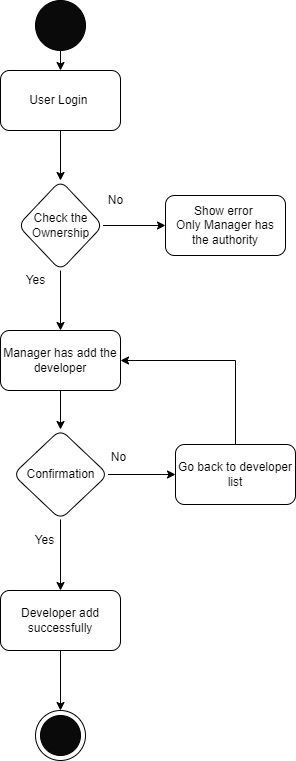
\includegraphics[scale=0.7]{./diagrams/Activity Diagram/ad-13.png}
    \caption{Activity diagram of UC-13}
    \label{fig:act-13}

\end{figure}


\textbf{Cyclomatic Complexity}

M= E+N + 2(P)

E= number of edges

N= number of nodes

P= number of paths

E= 9,
N= 9,
P= 1,

M= 9-9+2(1)= 2

\begin{figure}[H]
    \centering
    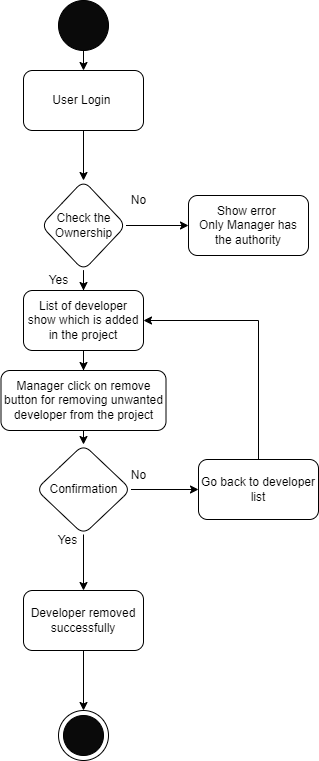
\includegraphics[scale=0.7]{./diagrams/Activity Diagram/ad-14.png}
    \caption{Activity diagram of UC-14}
    \label{fig:act-14}

\end{figure}


\textbf{Cyclomatic Complexity}

M= E+N + 2(P)

E= number of edges

N= number of nodes

P= number of paths

E= 10,
N= 10,
P= 1,

M= 10-10+2(1)= 2

\begin{figure}[H]
    \centering
    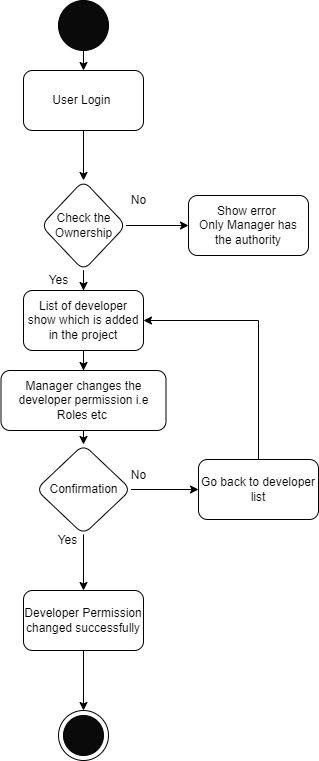
\includegraphics[scale=0.7]{./diagrams/Activity Diagram/ad-15.png}
    \caption{Activity diagram of UC-15}
    \label{fig:act-15}

\end{figure}


\textbf{Cyclomatic Complexity}

M= E+N + 2(P)

E= number of edges

N= number of nodes

P= number of paths

E= 10,
N= 10,
P= 1,

M= 10-10+2(1)= 2

\begin{figure}[H]
    \centering
    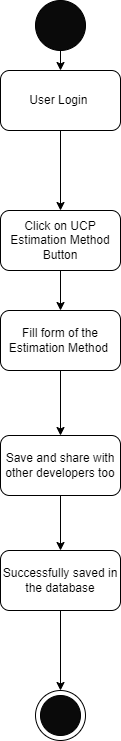
\includegraphics[scale=0.7]{./diagrams/Activity Diagram/ad-16.png}
    \caption{Activity diagram of UC-16}
    \label{fig:act-16}

\end{figure}


\textbf{Cyclomatic Complexity}

M= E+N + 2(P)

E= number of edges

N= number of nodes

P= number of paths

E= 6,
N= 7,
P= 1,

M= 6-7+2(1)= 1

\begin{figure}[H]
    \centering
    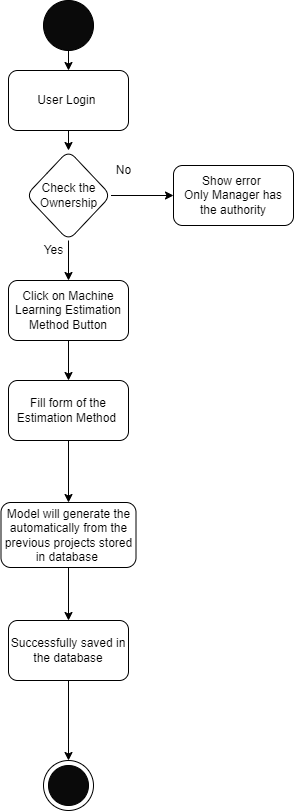
\includegraphics[scale=0.7]{./diagrams/Activity Diagram/ad-17.png}
    \caption{Activity diagram of UC-17}
    \label{fig:act-17}

\end{figure}

\textbf{Cyclomatic Complexity}

M= E+N + 2(P)

E= number of edges

N= number of nodes

P= number of paths

E= 8,
N= 9,
P= 1,

M= 8-9+2(1)= 1

\begin{figure}[H]
    \centering
    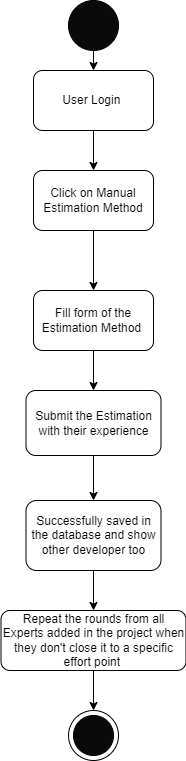
\includegraphics[scale=0.7]{./diagrams/Activity Diagram/ad-18.png}
    \caption{Activity diagram of UC-18}
    \label{fig:act-18}

\end{figure}


\textbf{Cyclomatic Complexity}

M= E+N + 2(P)

E= number of edges

N= number of nodes

P= number of paths

E= 7,
N= 8,
P= 1,

M= 7-8+2(1)= 1

\begin{figure}[H]
    \centering
    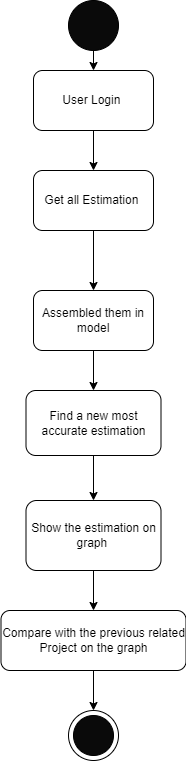
\includegraphics[scale=0.7]{./diagrams/Activity Diagram/ad-19.png}
    \caption{Activity diagram of UC-19}
    \label{fig:act-19}

\end{figure}

\textbf{Cyclomatic Complexity}

M= E+N + 2(P)

E= number of edges

N= number of nodes

P= number of paths

E= 7,
N= 8,
P= 1,

M= 7-8+2(1)= 1

\begin{figure}[H]
    \centering
    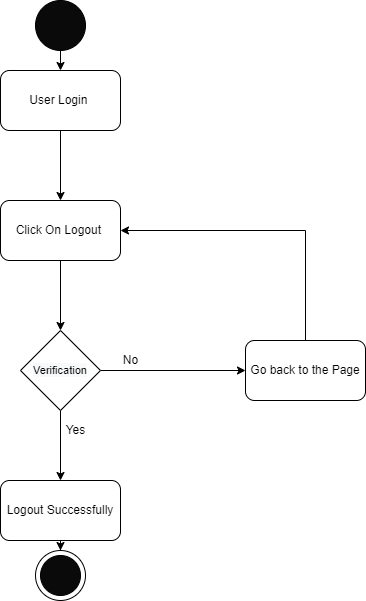
\includegraphics[scale=0.7]{./diagrams/Activity Diagram/ad-20.png}
    \caption{Activity diagram of UC-20}
    \label{fig:act-20}

\end{figure}


\textbf{Cyclomatic Complexity}

M= E+N + 2(P)

E= number of edges

N= number of nodes

P= number of paths

E= 7,   N= 7,   P= 1,

M= 7-7+2(1)= 2


% Path Coverage
\subsubsection{ Path Coverage}
Path coverage tests all the paths of the program. This is a comprehensive technique which ensures
that all the paths of the program are traversed at least once.
\subsubsection{ Statement Coverage}
This technique requires every possible statement in the code to be tested at least once during the
testing process of software engineering.

\subsubsection{ Branch Coverage}
This technique checks every possible path (if-else and other conditional loops) of a software
application.

\subsection{Performance Testing}
Performance tests help to determine a system`s and application`s limitations, as well as the maximum
number of active users utilizing the application throughout servers. The Performance Test Plan and
Results is a combined document designed to more closely integrate performance test planning and
reporting.

\subsection{Load Testing}
Load testing is a technique used to determine the number of users that can be used to access a system.
The load testing plan is a document designed to more closely integrate load testing planning and
reporting.

\subsection{Stress Testing}
Stress Testing is a type of software testing that verifies stability and reliability of software application.
The goal of Stress testing is measuring software on its robustness and error handling capabilities
under extremely heavy load conditions and ensuring that software doesn`t crash under crunch
situations.
\subsection{Regression Testing}
Regression Testing is a type of software testing to confirm that a recent program or code change has
not adversely affected existing features.